\documentclass[11pt]{article}

\usepackage[margin=1in]{geometry}
\usepackage{amsmath}
\usepackage{array}
\usepackage{graphicx}
\usepackage{float}
\usepackage[colorlinks=true,linkcolor=blue,urlcolor=blue,citecolor=blue]{hyperref}

\title{Gradient-Descent IMF with Lookup-Grid Robust Scores}
\author{}
\date{}

\begin{document}
\maketitle

\section{Task}

The notebook \href{https://github.com/mkuziuk/imf/blob/main/gd_irmf.ipynb}{gd\_irmf.ipynb}
implements a small demonstration of intrinsic multiscale filtering (IMF) for a
one-dimensional noisy signal. As in \texttt{IMF.pdf}, the observation is written as
\[
Y_t = X_t + \varepsilon_t,
\]
where \(X_t\) is the underlying signal and \(\varepsilon_t\) is noise, possibly with
contamination.

At IMF stage \(k\), the current residual \(Y^{(k)}\) is locally smoothed by solving
one scalar contrast problem at every time point:
\[
\widetilde S_t^{(k)}
= \operatorname{arginf}_x
\sum_u \rho_H\left(Y_u^{(k)} - x\right)K_{h_k}(t-u).
\]
The extracted component \(\widetilde S^{(k)}\) is then subtracted from the current
residual:
\[
Y_t^{(k+1)} = Y_t^{(k)} - \widetilde S_t^{(k)}.
\]
This recursion is sequential across IMF stages, but the local contrast fits inside one
fixed stage are independent and can be evaluated in parallel.

The notebook uses the Epanechnikov kernel
\[
K(u) = \frac{3}{4}(1 - |u|)^2_+,
\]
with normalized discrete weights inside each local window. In the notation of
\texttt{IMF.pdf}, \(h_k\) is the bandwidth or half-width: the contributing points
lie in \([t-h_k,t+h_k]\). In the notebook, however, \texttt{window\_size} is the
number of discrete sampled points in the symmetric window. Thus
\[
\texttt{window\_size}=2R+1,
\]
where \(R\) is the discrete radius in grid-index steps. The first notebook window is
\(501=2\cdot 250+1\), so it has discrete radius \(R=250\). On the normalized grid
\([0,1]\) with \(1000\) points, this corresponds to a continuous half-width of
approximately \(250/999\). Later window sizes are decreased by approximately
\(\sqrt{2}\) until the minimum window size is reached.

The main notebook parameters are summarized below.

\begin{table}[H]
\centering
\small
\begin{tabular}{@{}>{\raggedright\arraybackslash}p{0.18\linewidth}
>{\raggedright\arraybackslash}p{0.29\linewidth}
>{\raggedright\arraybackslash}p{0.45\linewidth}@{}}
\hline
Symbol / name & Notebook value & Meaning \\
\hline
\(n\) & \(\texttt{1000}\) & Number of sample points. \\
\(t\) & \([0,1]\) & Normalized design interval. \\
\(\sigma\) & \(\texttt{0.2}\) & Gaussian noise scale. \\
\(H\) & \(2\sigma = 0.4\) & Robust contrast smoothing scale. \\
\(K\) & Epanechnikov & Kernel \(K(u)=\frac{3}{4}(1-|u|)^2_+\). \\
\(h_k\) & radius / bandwidth & PDF half-width; notebook radius is
\(R_k=(\texttt{window\_size}_k-1)/2\). \\
first window & \(\texttt{window\_size}=501,\ R=250,\ h_1\approx250/999\) &
First full discrete window and corresponding radius. \\
\(a\) & \(\sqrt{2}\approx1.414\) & Window shrink factor used by
\texttt{make\_window\_schedule}. \\
minimum window & \(\texttt{31}\) points, \(R=15\) & Stopping window size and
final discrete radius. \\
lookup grid & \(\texttt{zmax}=8,\ \texttt{num}=4097\) & Grid for score and
exponential lookup. \\
\(\eta\) & \(0.95H/\sqrt{2/\pi}\approx0.476\) & Gradient-descent step size. \\
optimization & \(\texttt{max\_iter}=60,\ \texttt{tol}=10^{-6}\) & Local fit
iteration limit and stopping tolerance. \\
parallelism / boundary & \(\texttt{max\_workers}=12,\ \texttt{boundary}=\texttt{wrap}\) &
Parallel chunking and boundary handling. \\
contamination & probability \(0.2\), scale \(0.2\), seed \(777\) & Synthetic
one-sided contamination settings. \\
\hline
\end{tabular}
\caption{Main parameters used in \texttt{gd\_irmf.ipynb}.}
\end{table}

\begin{figure}[H]
\centering
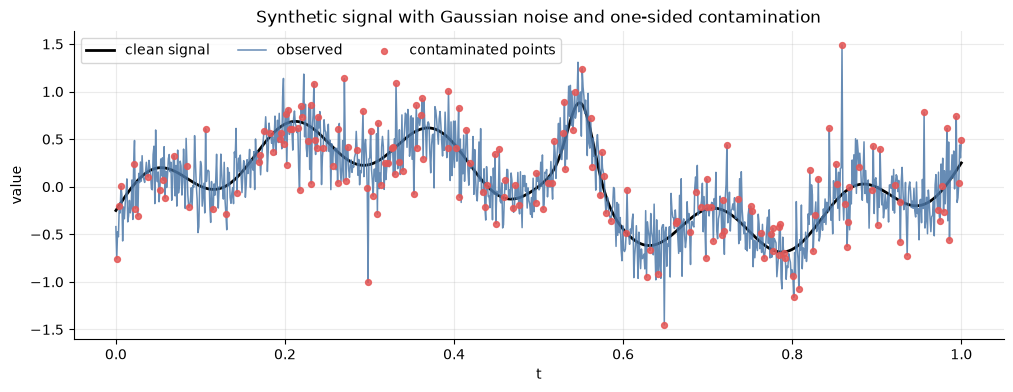
\includegraphics[width=\linewidth]{figures/gd_irmf/observed_signal.png}
\caption{Synthetic observation used in the notebook, with the clean signal and
contaminated points shown for reference.}
\end{figure}

\section{Robust Contrast and Lookup Grid}

The smooth robust contrast used in the notebook is
\[
\rho_H(r)
= r\,\operatorname{erf}\left(\frac{r}{\sqrt{2}H}\right)
+ \sqrt{\frac{2}{\pi}}H
\exp\left(-\frac{r^2}{2H^2}\right),
\]
with score function
\[
\psi_H(r) = \rho_H'(r)
= \operatorname{erf}\left(\frac{r}{\sqrt{2}H}\right).
\]
Gradient descent repeatedly evaluates this score on large local-window matrices.
Rather than recomputing the error function and exponential for every residual value,
the notebook uses the scaled residual
\[
z = \frac{r}{H}
\]
and precomputes a lookup table over
\[
z_i = -8 + i\Delta z,\qquad
\Delta z = \frac{16}{4096},\qquad i=0,\ldots,4096.
\]
The stored arrays are
\[
s_i = \operatorname{erf}\left(\frac{z_i}{\sqrt{2}}\right),
\qquad
e_i = \exp\left(-\frac{z_i^2}{2}\right).
\]
For a new residual \(r\), the code computes \(z=r/H\) and evaluates \(s(z)\) and
\(e(z)\) by linear interpolation. Outside the grid, the score is saturated to
\(-1\) or \(1\), and the exponential tail is set to \(0\). This is accurate because
\[
\exp(-8^2/2) \approx 1.27 \times 10^{-14}.
\]
In the current run, the maximum lookup errors on a dense validation grid are about
\(9.23\times 10^{-7}\) for the score and \(1.91\times 10^{-6}\) for the exponential.

\begin{figure}[H]
\centering
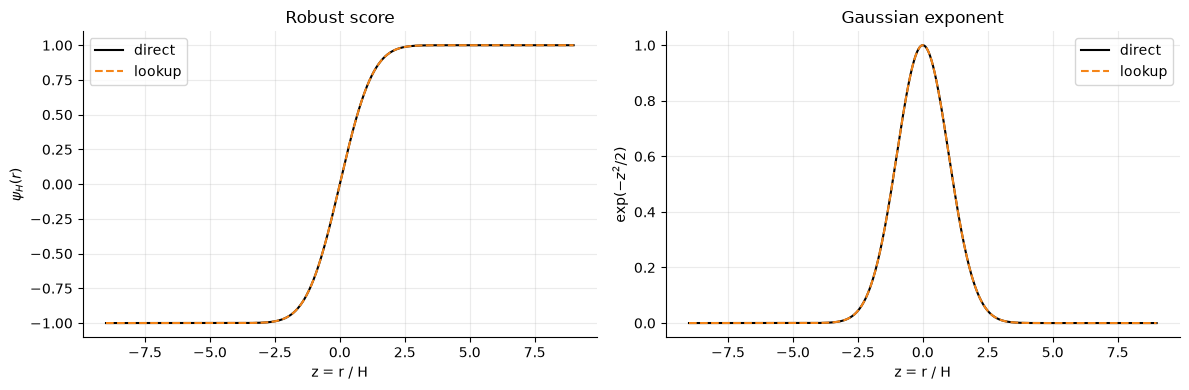
\includegraphics[width=\linewidth]{figures/gd_irmf/lookup_grid.png}
\caption{Direct formulas compared with lookup-grid interpolation for the robust score
and Gaussian exponent.}
\end{figure}

\section{Notebook Review}

For a fixed stage \(k\), each row of the local window matrix is a separate
one-dimensional optimization problem. The gradient-descent update is
\[
x_t^{(m+1)}
= x_t^{(m)}
+ \eta\sum_u w_{t,u}
\psi_H\left(Y_u^{(k)} - x_t^{(m)}\right),
\]
where \(w_{t,u}\) are normalized Epanechnikov weights. The implementation vectorizes
many local fits at once and can split the window matrix into chunks processed by
multiple workers.

To make the sequential residual updates comparable across the full stage grid, the
notebook uses one shared \(y\)-axis range for every panel in this grid. Other
notebook plots keep their own automatic vertical scaling.

\begin{figure}[p]
\centering
\makebox[\linewidth][c]{%
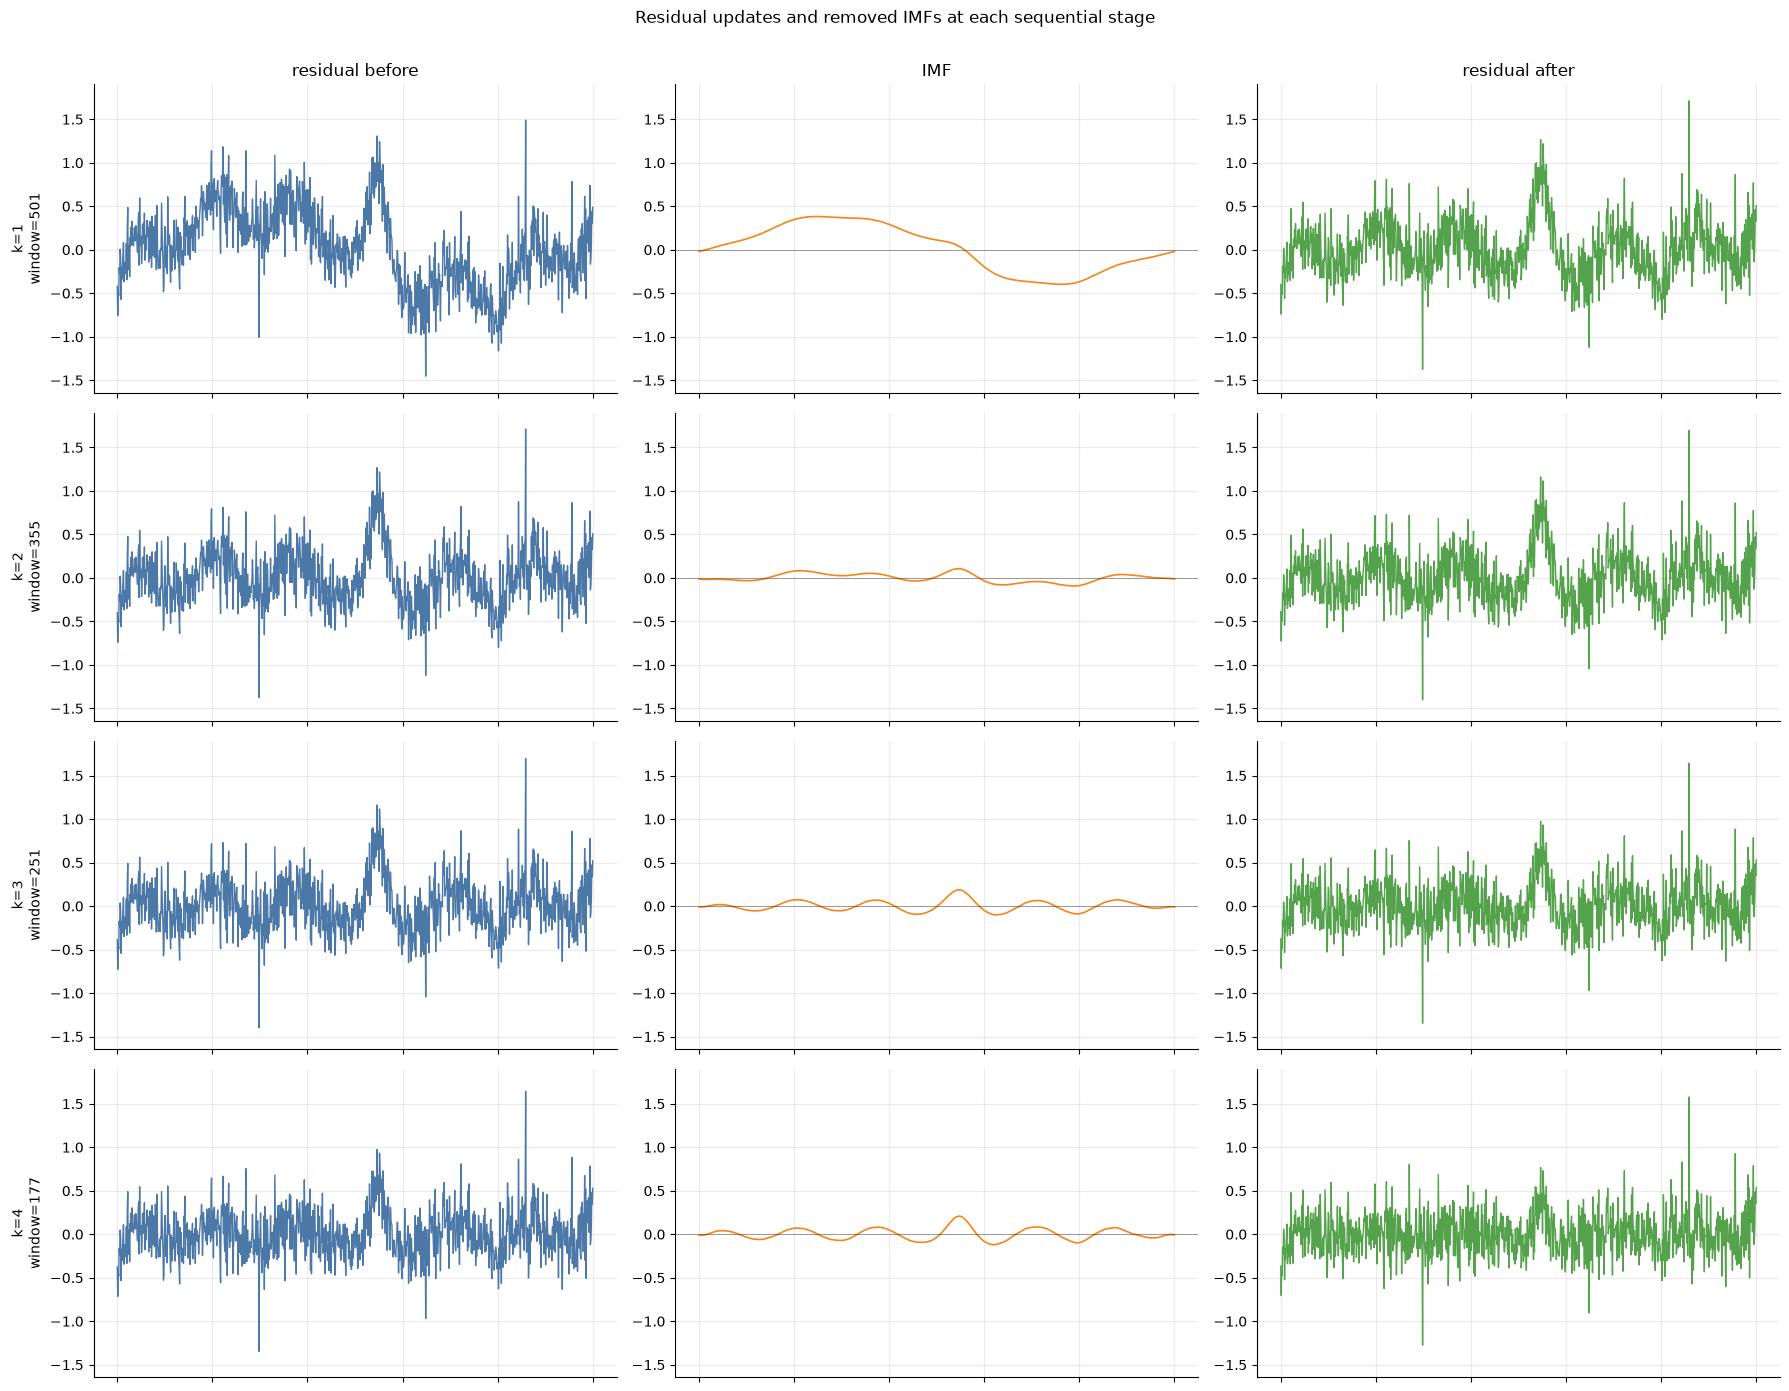
\includegraphics[width=1.12\linewidth,height=0.84\textheight,keepaspectratio]{figures/gd_irmf/imf_stages_top.png}%
}
\caption{Residual updates and removed IMFs for the first half of the stage grid.
Each row shows the residual before filtering, the removed IMF, and the residual
after subtraction.}
\end{figure}

\begin{figure}[p]
\centering
\makebox[\linewidth][c]{%
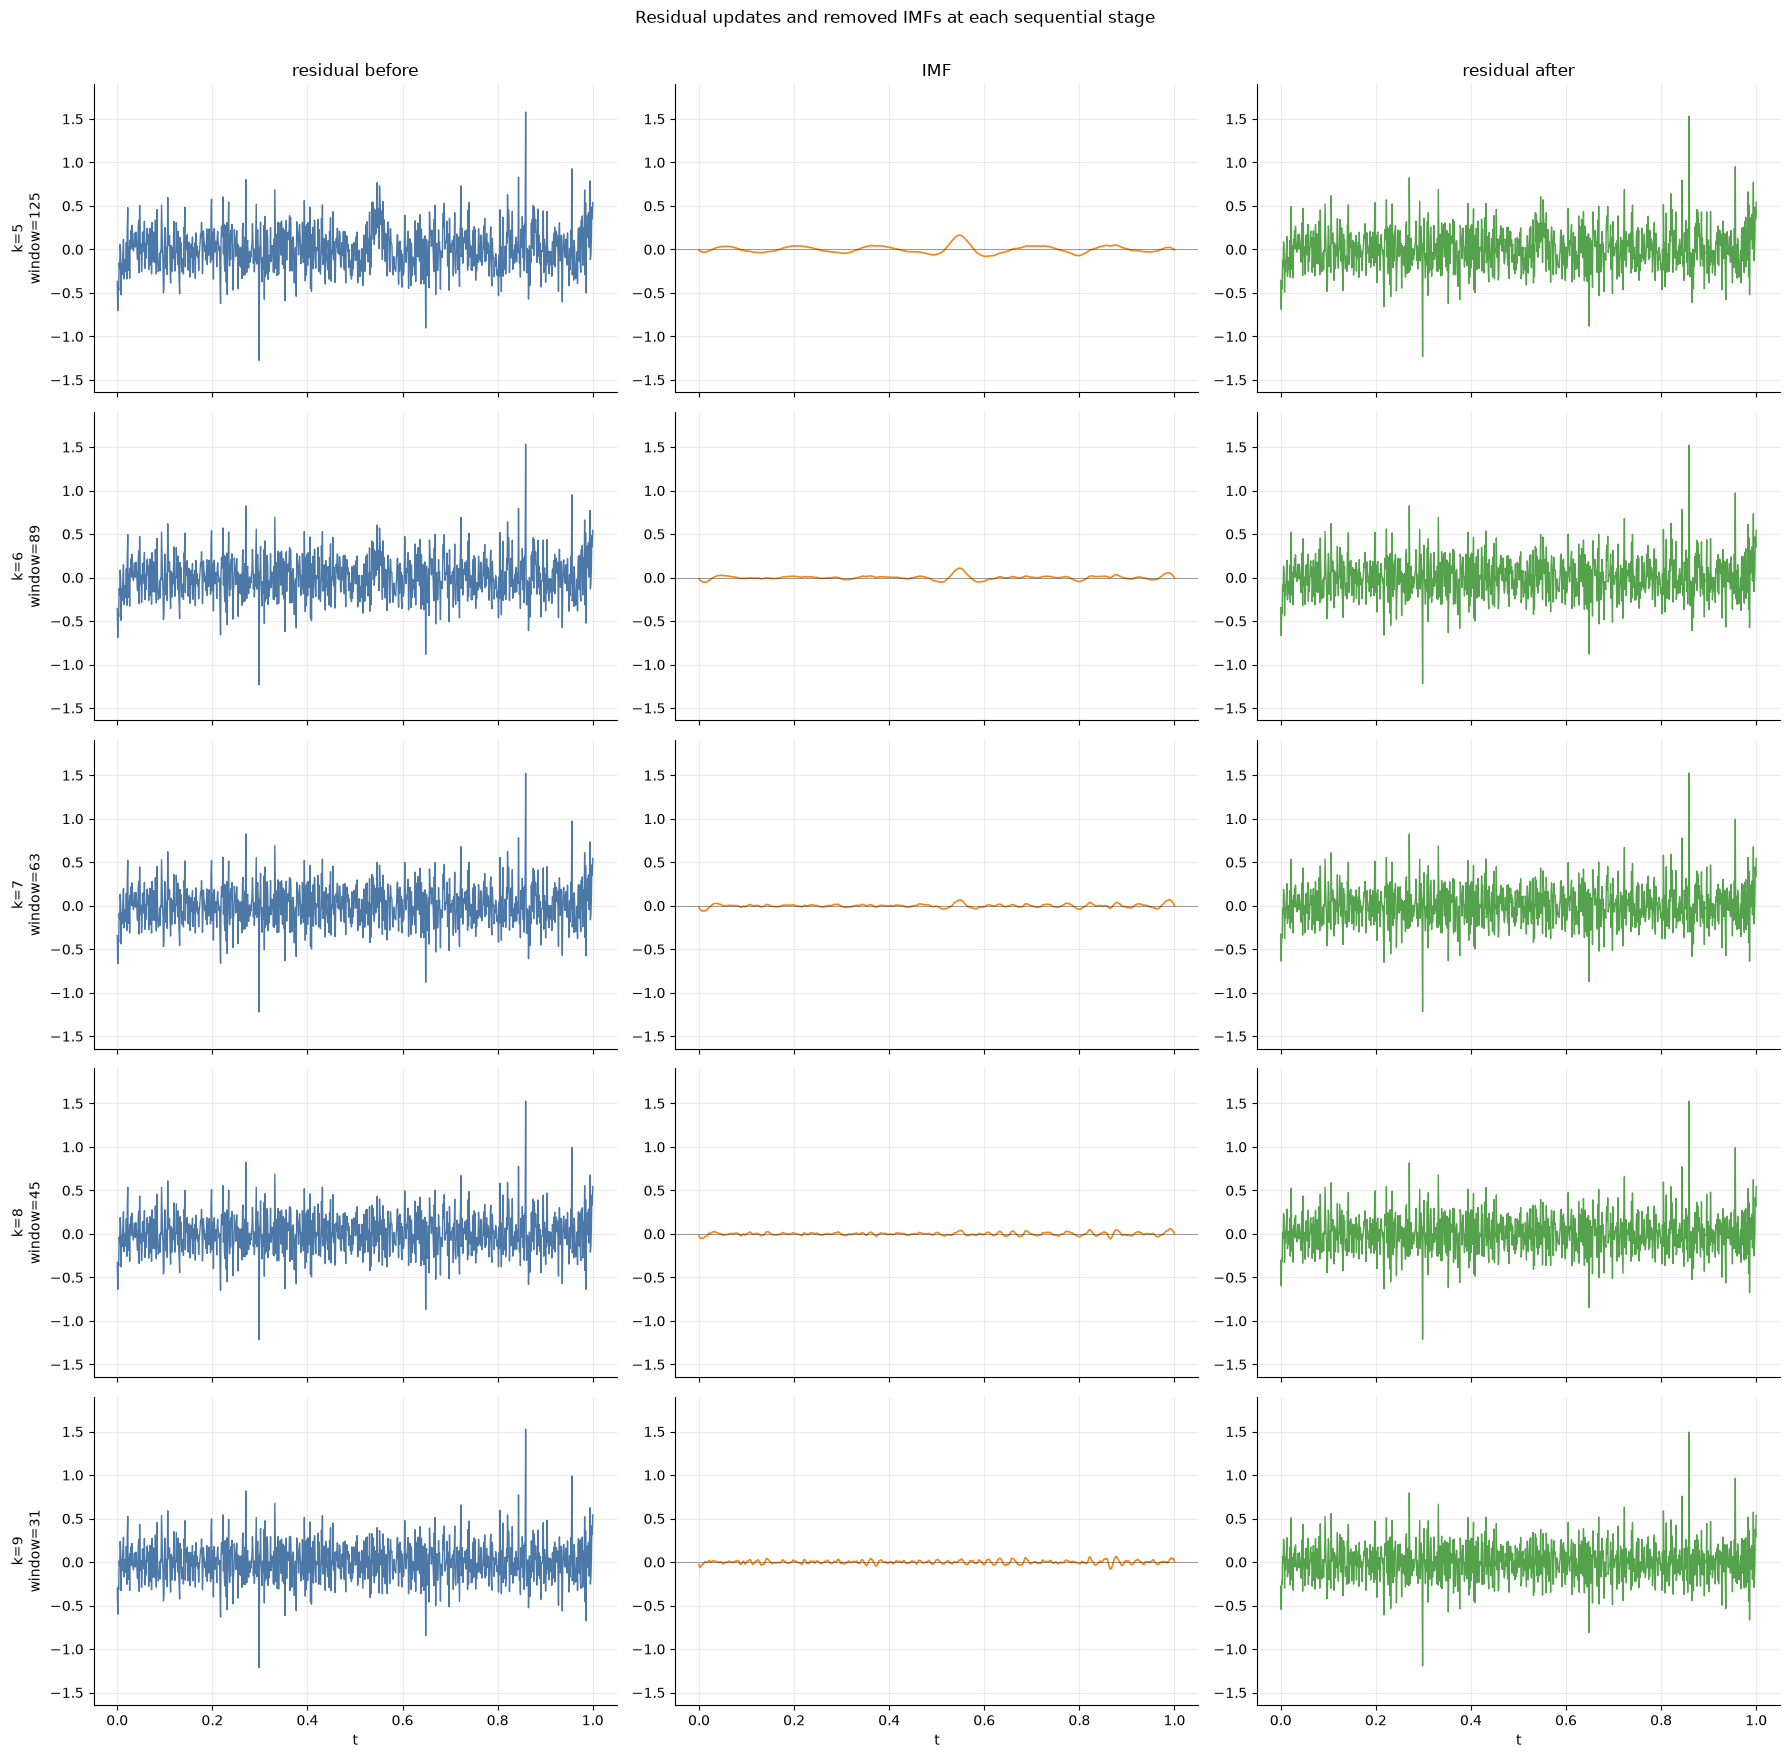
\includegraphics[width=1.12\linewidth,height=0.84\textheight,keepaspectratio]{figures/gd_irmf/imf_stages_bottom.png}%
}
\caption{Residual updates and removed IMFs for the second half of the stage grid.
Both halves use the same shared \(y\)-axis limits from the notebook.}
\end{figure}

The decomposition reconstructs the observation up to numerical precision:
\[
\left\|Y - \left(\sum_k \widetilde S^{(k)} + Y^{(\mathrm{final})}\right)\right\|_\infty
\approx 2.22\times 10^{-16}.
\]
For the current synthetic example, the observation has RMSE about \(0.237\) relative
to the clean signal, while the sum of extracted IMFs has RMSE about \(0.065\) relative
to the clean signal. The correlation between the sum of IMFs and the clean signal is
about \(0.986\), and the final residual RMS is about \(0.218\).

\begin{figure}[H]
\centering
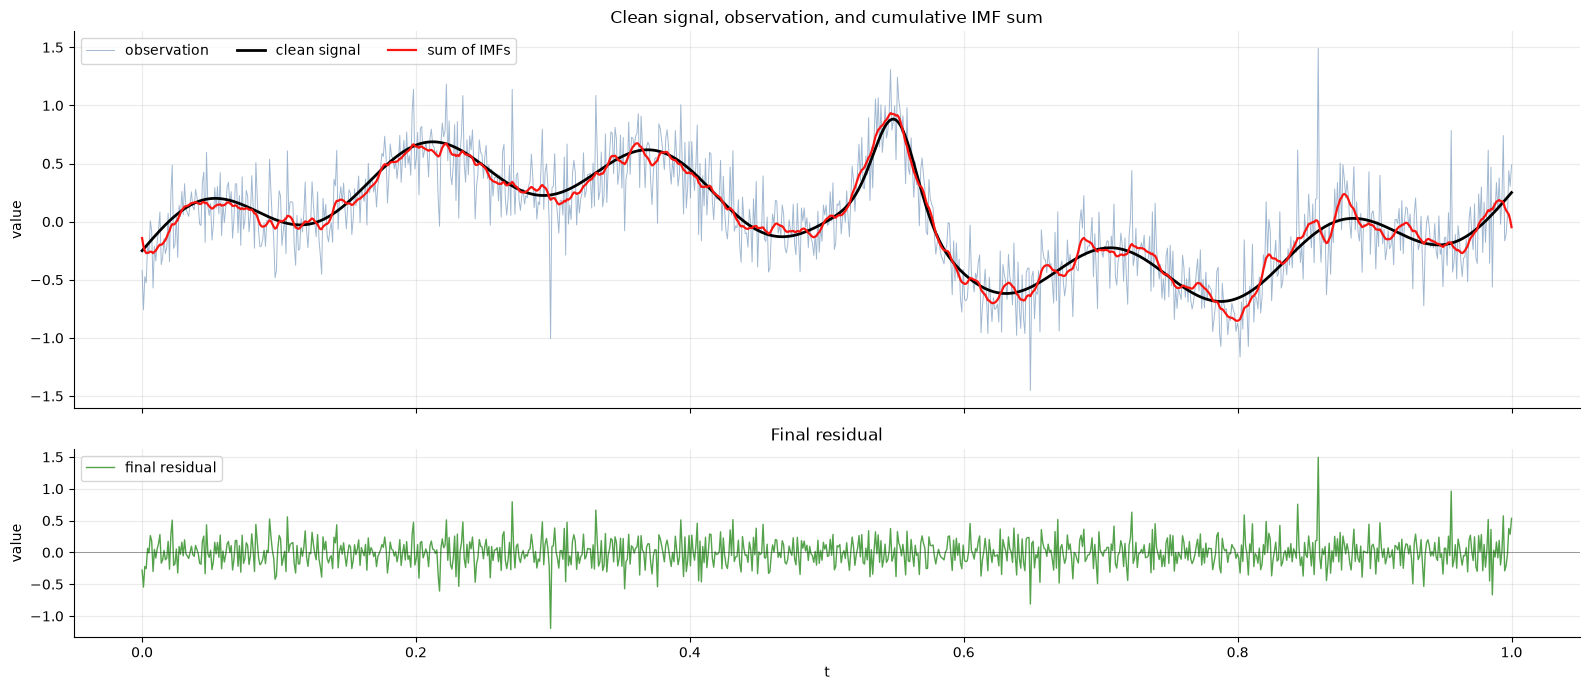
\includegraphics[width=\linewidth]{figures/gd_irmf/final_comparison.png}
\caption{The final notebook comparison overlays the noisy observation, clean signal,
and sum of IMFs, then shows the final residual separately.}
\end{figure}

\end{document}
